\documentclass{beamer}
\usepackage[tohoku,zh]{collegeBeamer}
% Set Japanese fonts using xeCJK
\usepackage{xeCJK}
\setCJKmainfont{Noto Serif CJK JP}       % Serif Japanese font
\setCJKsansfont{Noto Sans CJK JP}        % Sans-serif Japanese font
\setCJKmonofont{Noto Sans Mono CJK JP}   % Monospace Japanese font  
\definecolor{hrefcol}{RGB}{0, 0, 255} % Example: blue color
\usepackage{xcolor} % For defining and using custom colors
\usepackage{natbib} % Alternative with natbib

\usepackage{natbib}
\bibliographystyle{apalike}
\setbeamercovered{transparent}
\usepackage{xcolor}



% Add your bibliography file
\bibliography{references} % For natbib
\newcommand{\rfootnote}[1]{
  \addtocounter{framenumber}{-1}
  \begin{tikzpicture}[remember picture,overlay]
    \node[anchor=south east, inner sep=2.9mm, yshift=-1mm] at (current page.south east) {
      \begin{minipage}{0.55\textwidth} % Adjust width as needed
        \tiny % Decrease font size
        #1
      \end{minipage}
    };
  \end{tikzpicture}
  \addtocounter{framenumber}{1}
}

% Define the custom color
\definecolor{custompurple}{RGB}{62,21,134}

\setbeamercolor{block title}{bg=custompurple,fg=white} % White text on purple background
\setbeamercolor{block body}{bg=custompurple!10,fg=black} % Light purple background for body

% Define the new command for bold and colored text
\newcommand{\boldcolor}[1]{\textbf{\textcolor{custompurple}{#1}}}
% meta-data
\title{\textbf{意識・健康・ウェルビーイング研究会}}

\author{\textsc{呂沢宇}}
\institute{%
    \textit{東北大学}\\
    \textit{文学研究科 \hspace{0.2cm}  計算人文社会学専攻分野}}

\date{2025年3月3日}

% document body
\begin{document}

    \maketitle


    \begin{frame}{自己紹介}{\secname}

    \begin{itemize}
        \item \textbf{専門}：計算社会科学
        \item \textbf{所属}：東北大学文学研究科 \hspace{0.2cm}  計算人文社会学専攻分野
        \item SSM調査ビックデータタスクフォース
        \begin{itemize}
            \item 社会調査とビックデータの連携
            \item 計算的手法やビックデータ解析による社会調査の実施と分析に支援
        \end{itemize}
    \end{itemize}
    \end{frame}

    \begin{frame}{現在取り組んでいる研究}{オンライン空間における意見形成}
        \begin{columns}
        \begin{column}{0.5\textwidth}
                \begin{itemize}
                    \item 大規模なソーシャルメディアデータやオンラインニュースデータに基づく実証分析
                    \begin{itemize}
                          \item \textbf{自然言語処理によるテキストマイニング}
                          \item ネットワーク分析
                     \end{itemize}

                \end{itemize}
        \end{column}        
        \begin{column}{0.5\textwidth}
            \begin{figure}
            \centering
            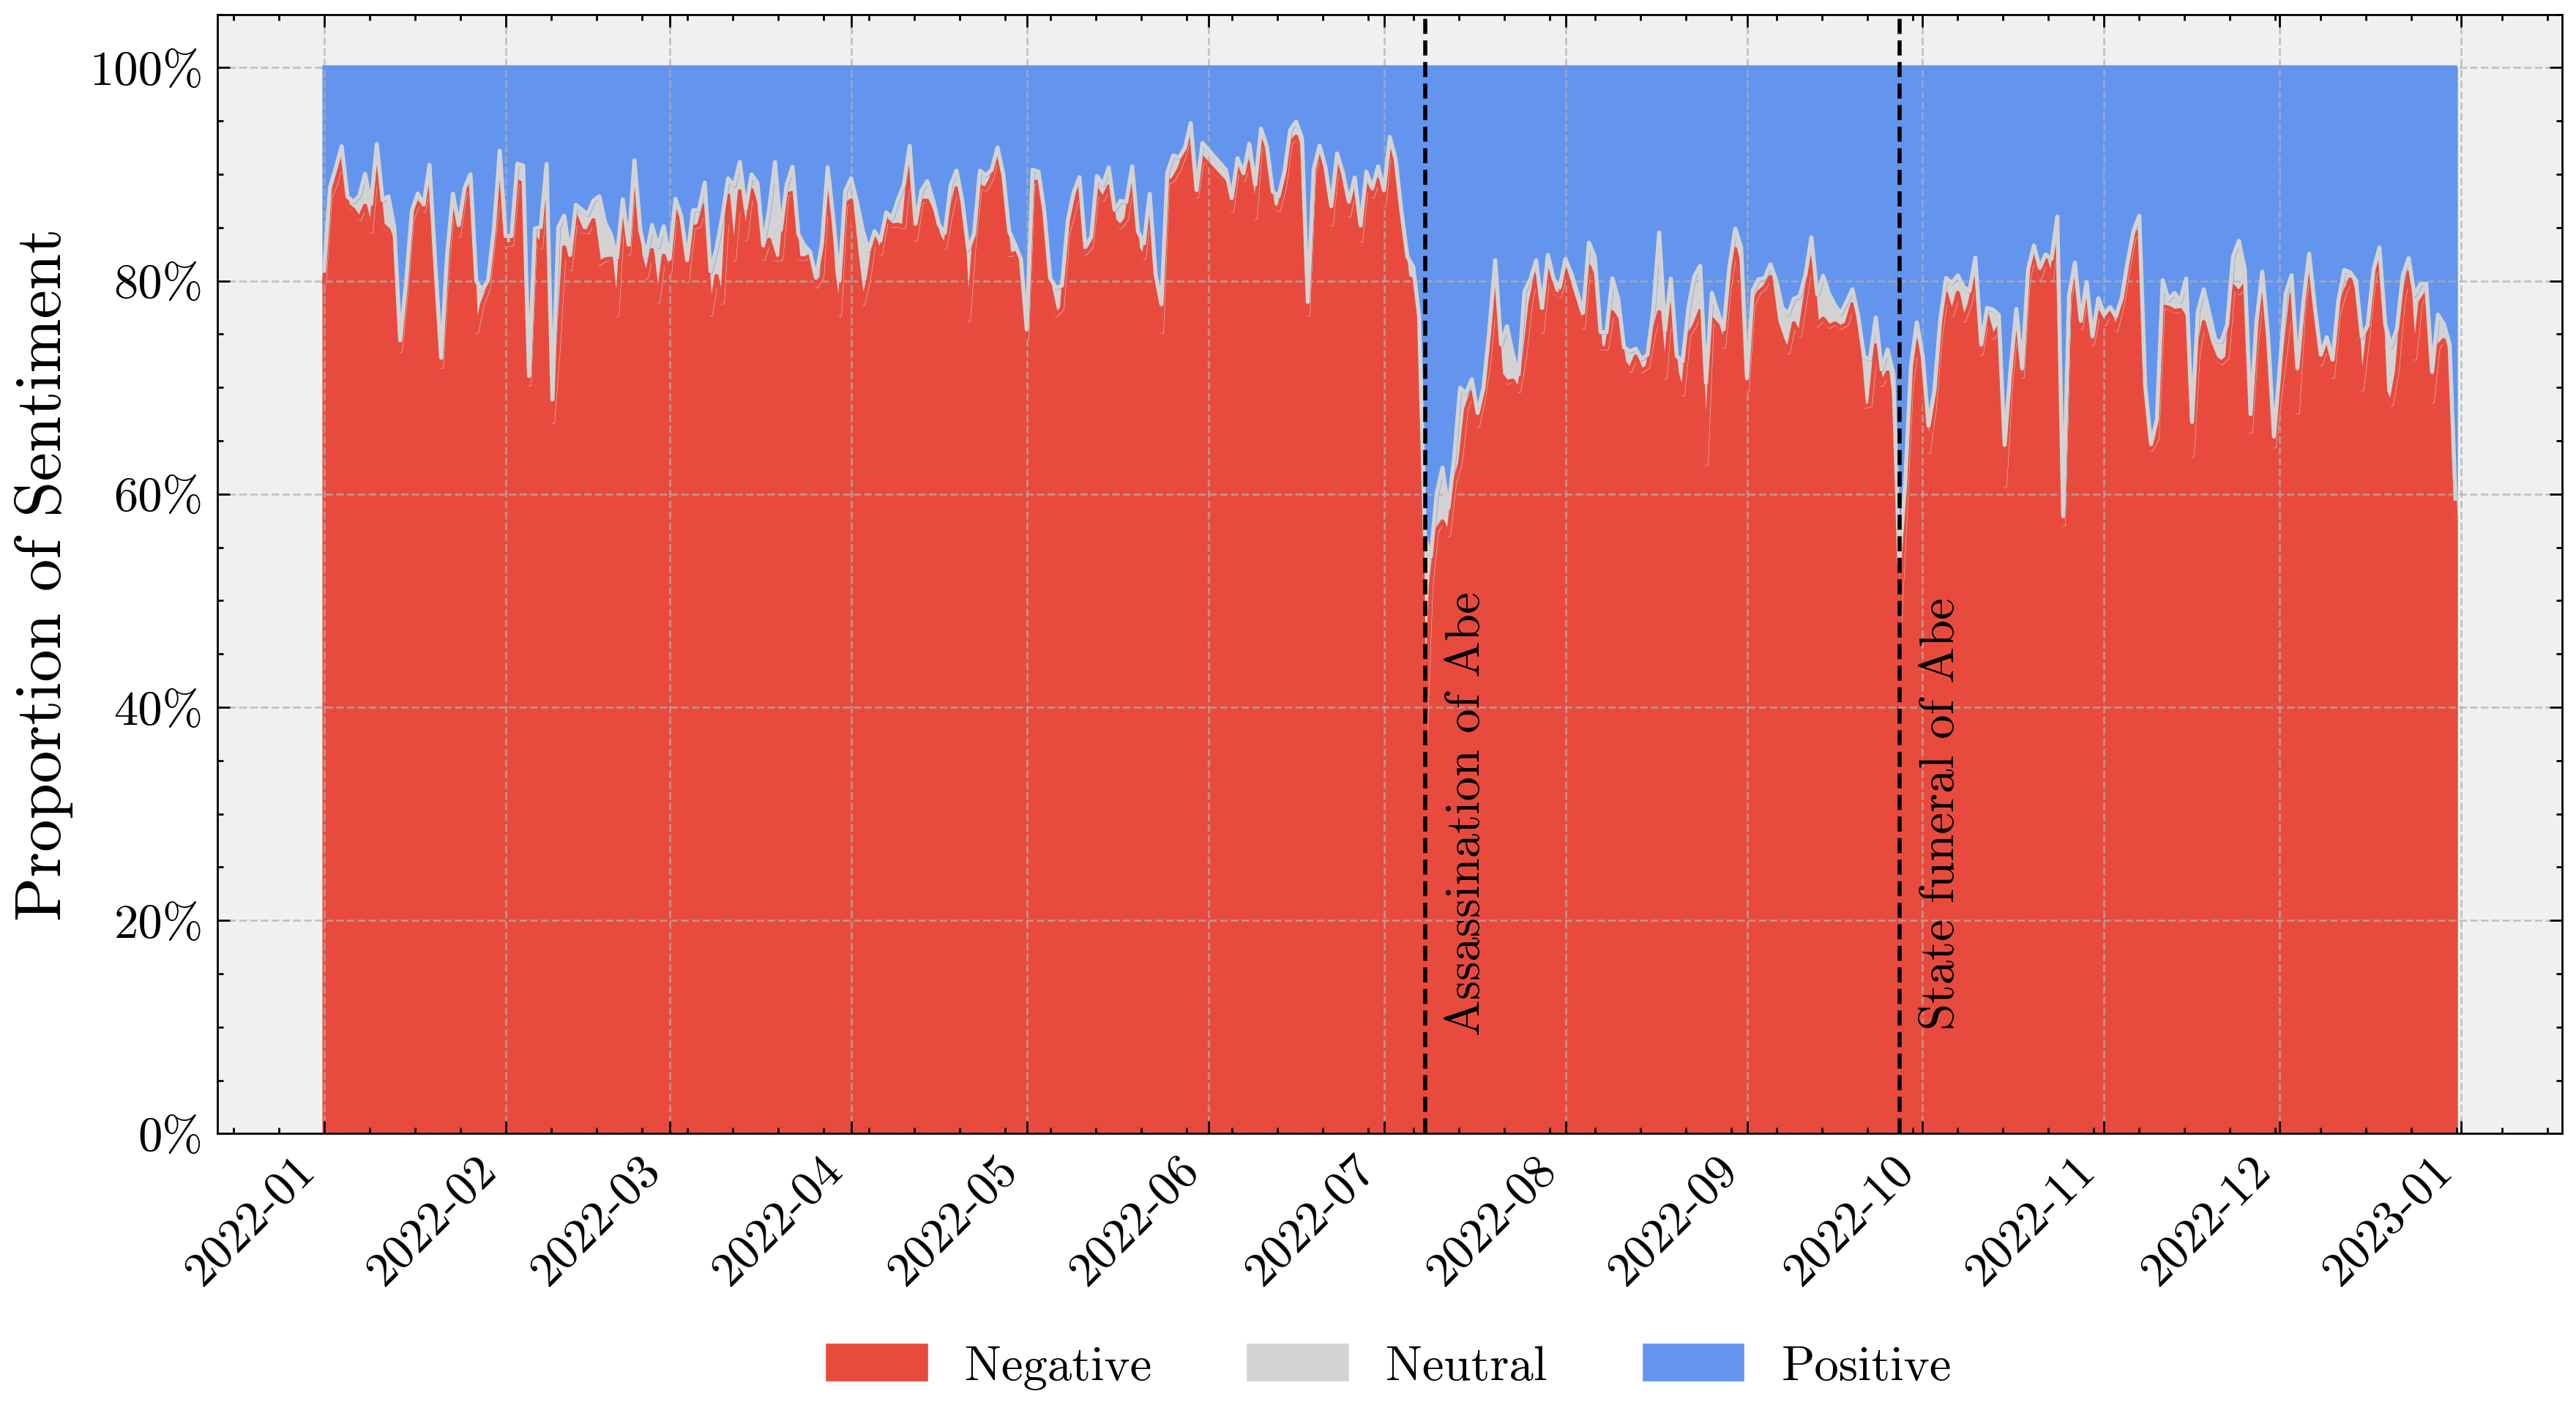
\includegraphics[width=\linewidth]{Figure/sentiment_over_time.png}
            \caption{ソーシャルメディアにおける長期的な意見変化}
            \label{fig:enter-label}
            \end{figure}
            \end{column}
        \end{columns}
    \end{frame}


    \begin{frame}{現在取り組んでいる研究}{モビリティデータによる社会的空間隔離の分析}
        \begin{columns}
        \begin{column}{0.5\textwidth}
                \begin{itemize}
                    \item \textbf{モビリティデータ}：モバイルセンサによる取得される位置情報
                    \pause
                    \item \textbf{社会的空間隔離}: 異なる社会集団が地理的に分離される
                    \begin{itemize}
                          \item 社会的分断
                          \item 機会の不平等
                     \end{itemize}

                \end{itemize}
        \end{column}        
        \begin{column}{0.5\textwidth}
            \begin{figure}
            \centering
            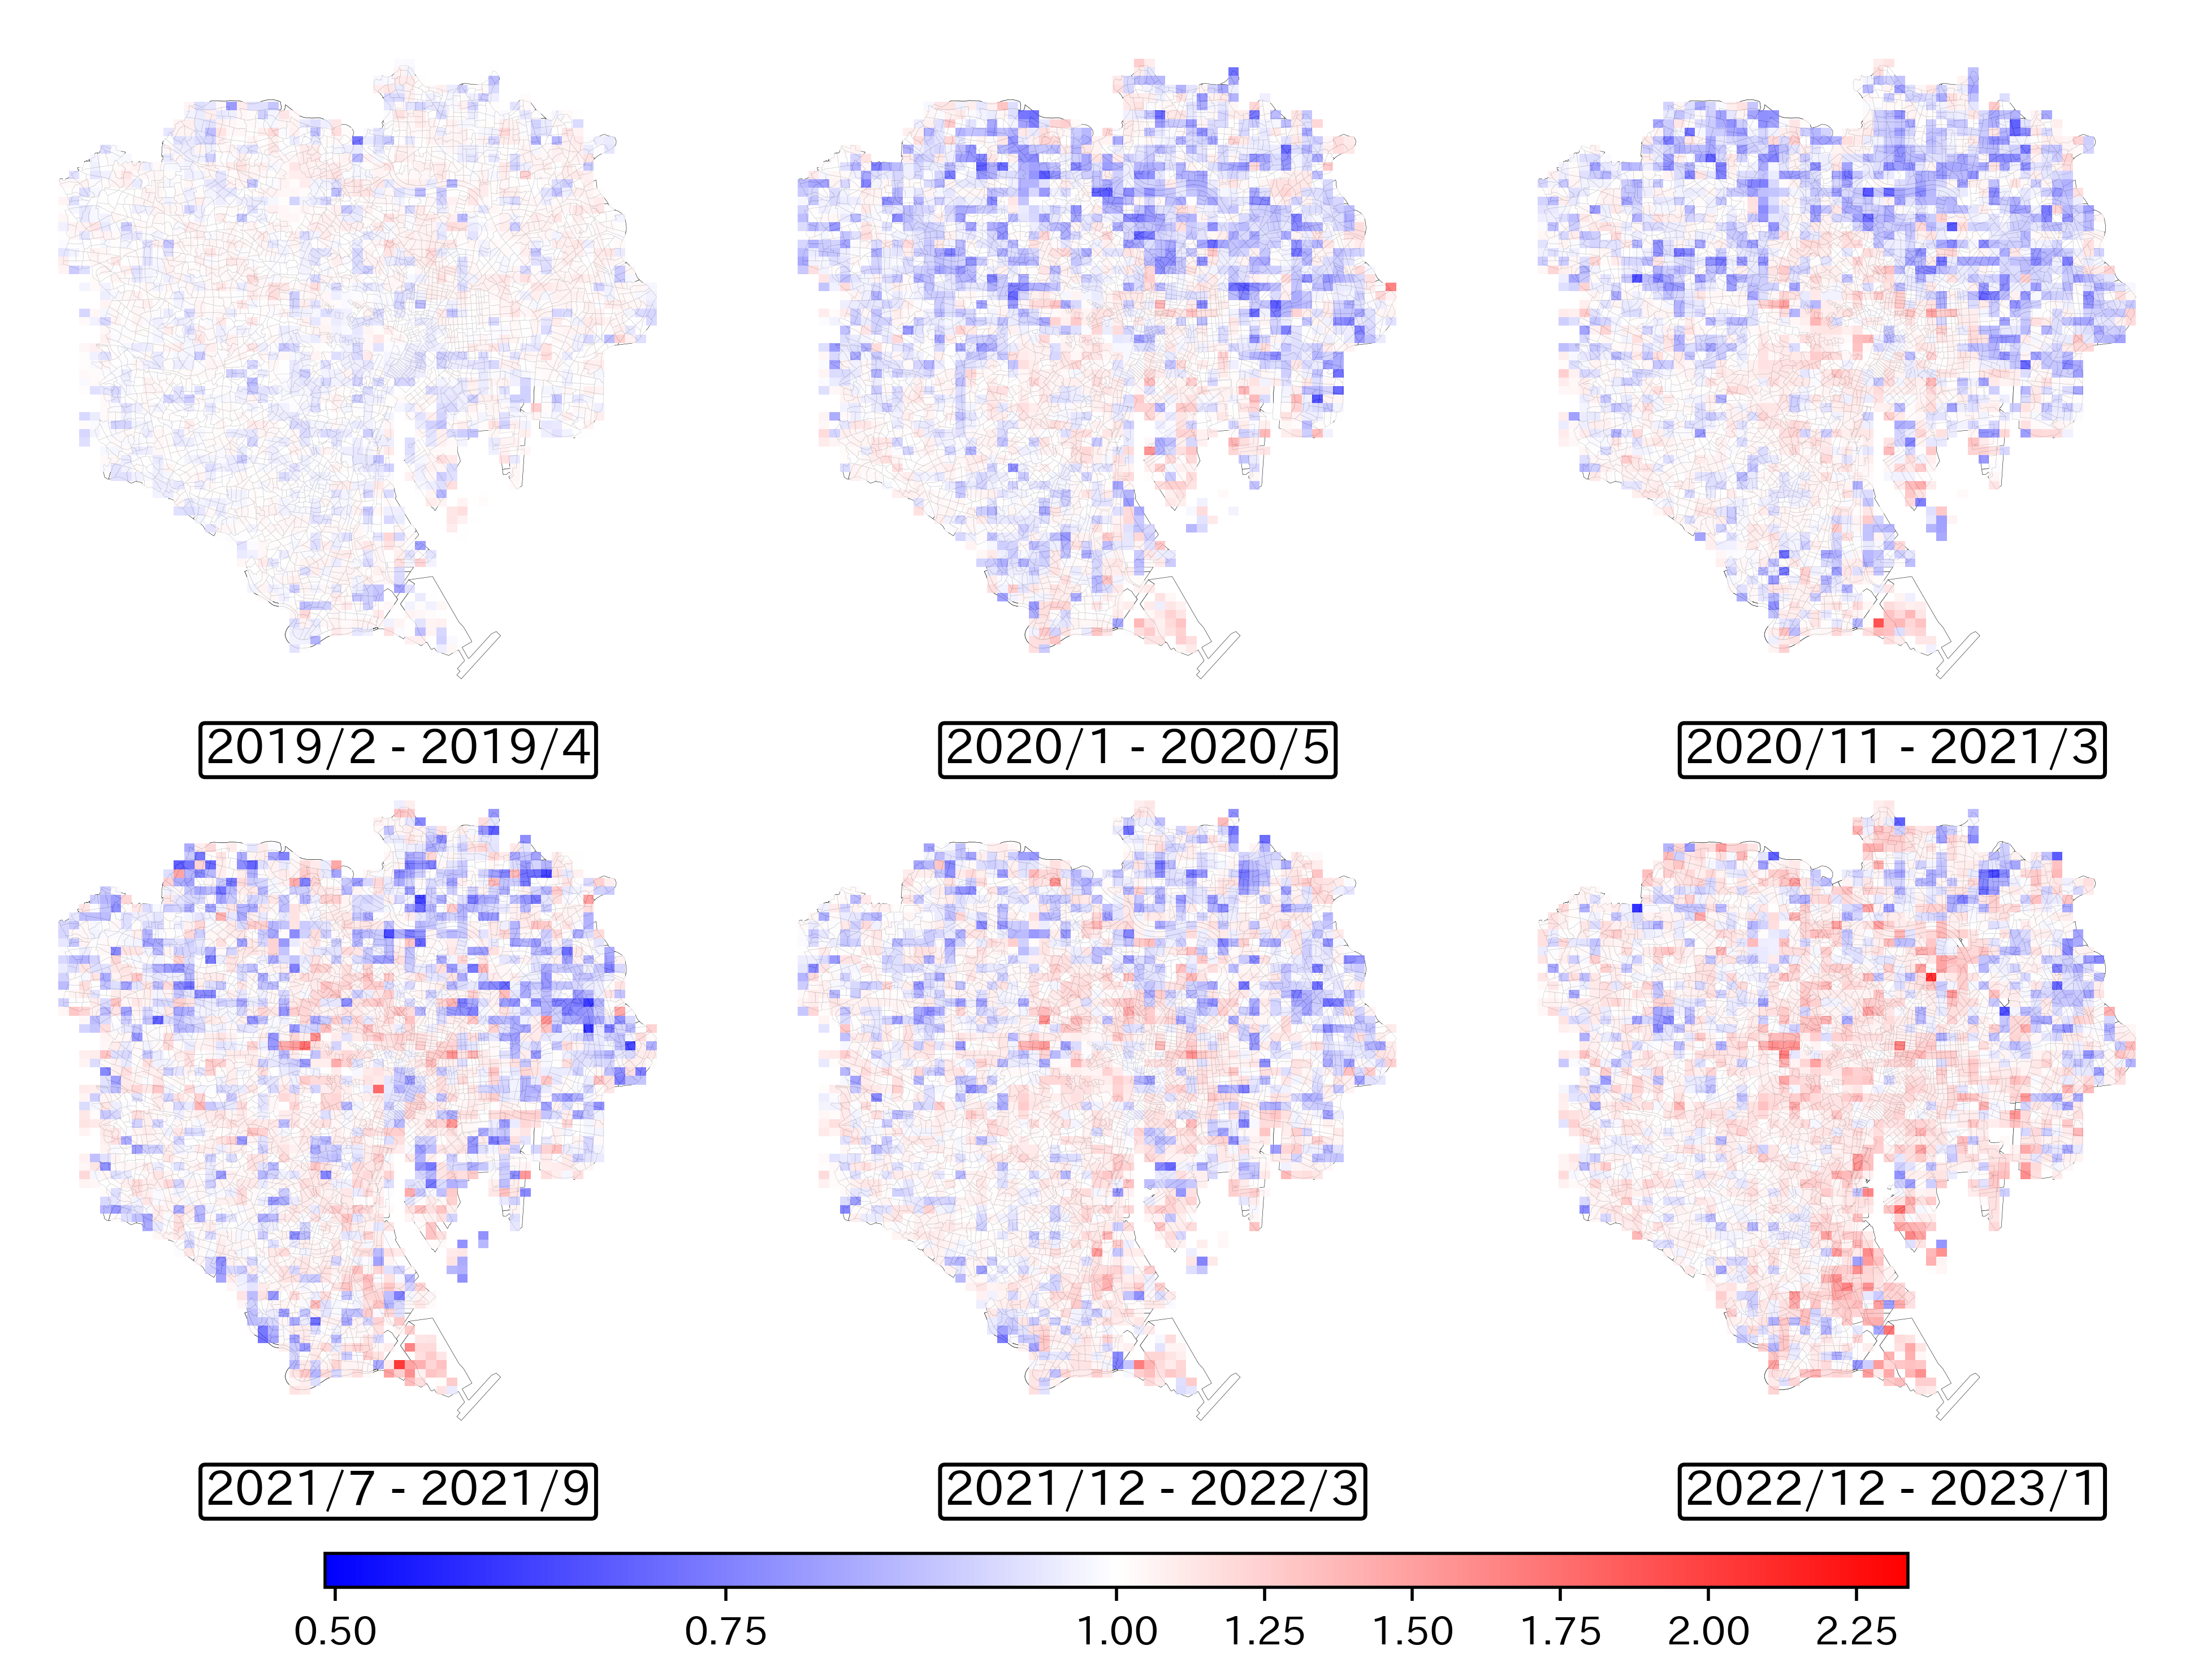
\includegraphics[width=\linewidth]{Figure/se_map.png}
            \caption{コロナにおける社会的空間隔離の推移}
            \label{fig:enter-label}
            \end{figure}
            \end{column}
        \end{columns}
    \end{frame}

\begin{frame}{現在取り組んでいる研究}{歴史資料に対するテキストマイニング}
    \begin{columns}
        \begin{column}{0.5\textwidth}
            \vspace{-0.5cm} % 调整文字和图像之间的间距
            \begin{minipage}[t][0.8\textheight][t]{\textwidth} % 设置统一高度
                \begin{itemize}
                    \item 歴史記録から天文・気象状況の特定と分析
                \end{itemize}
                \begin{figure}
                    \centering
                    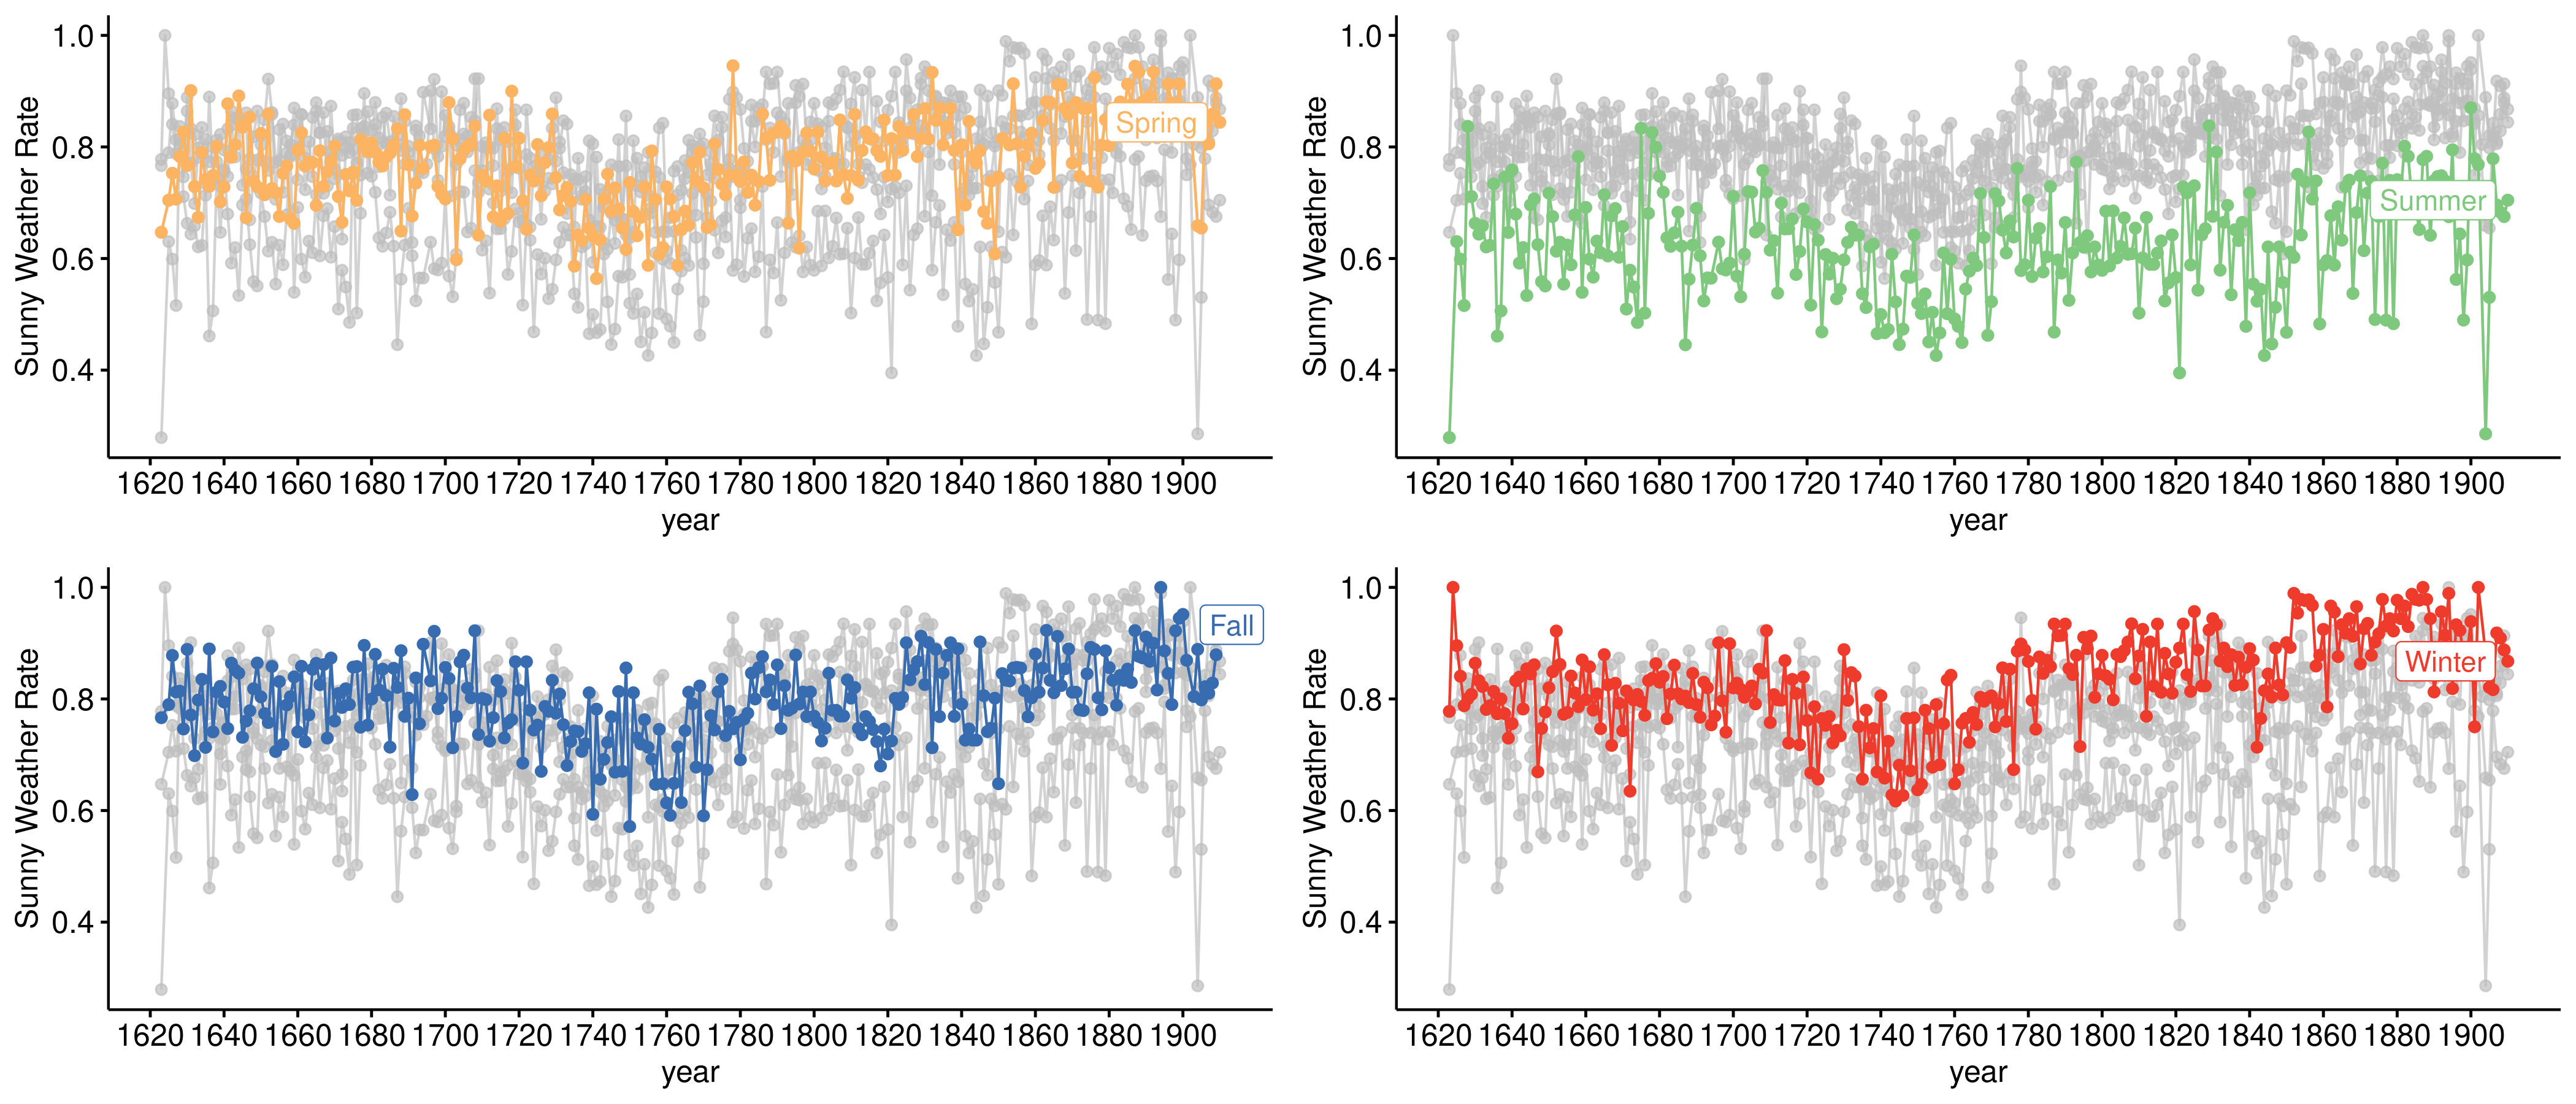
\includegraphics[width=0.9\linewidth]{Figure/p_rate.png}
                    \caption{歴史記録による特定した数百年間晴天率の推移}
                    \label{fig:enter-label}
                \end{figure}
            \end{minipage}
        \pause
        \end{column}
        \begin{column}{0.5\textwidth}
            \vspace{-0.5cm} % 调整文字和图像之间的间距
            \begin{minipage}[t][0.8\textheight][t]{\textwidth} % 设置统一高度
                \begin{itemize}
                    \item テキストによる集合表象・集合意識に対して定量的な測定
                \end{itemize}
                \begin{figure}
                    \centering
                    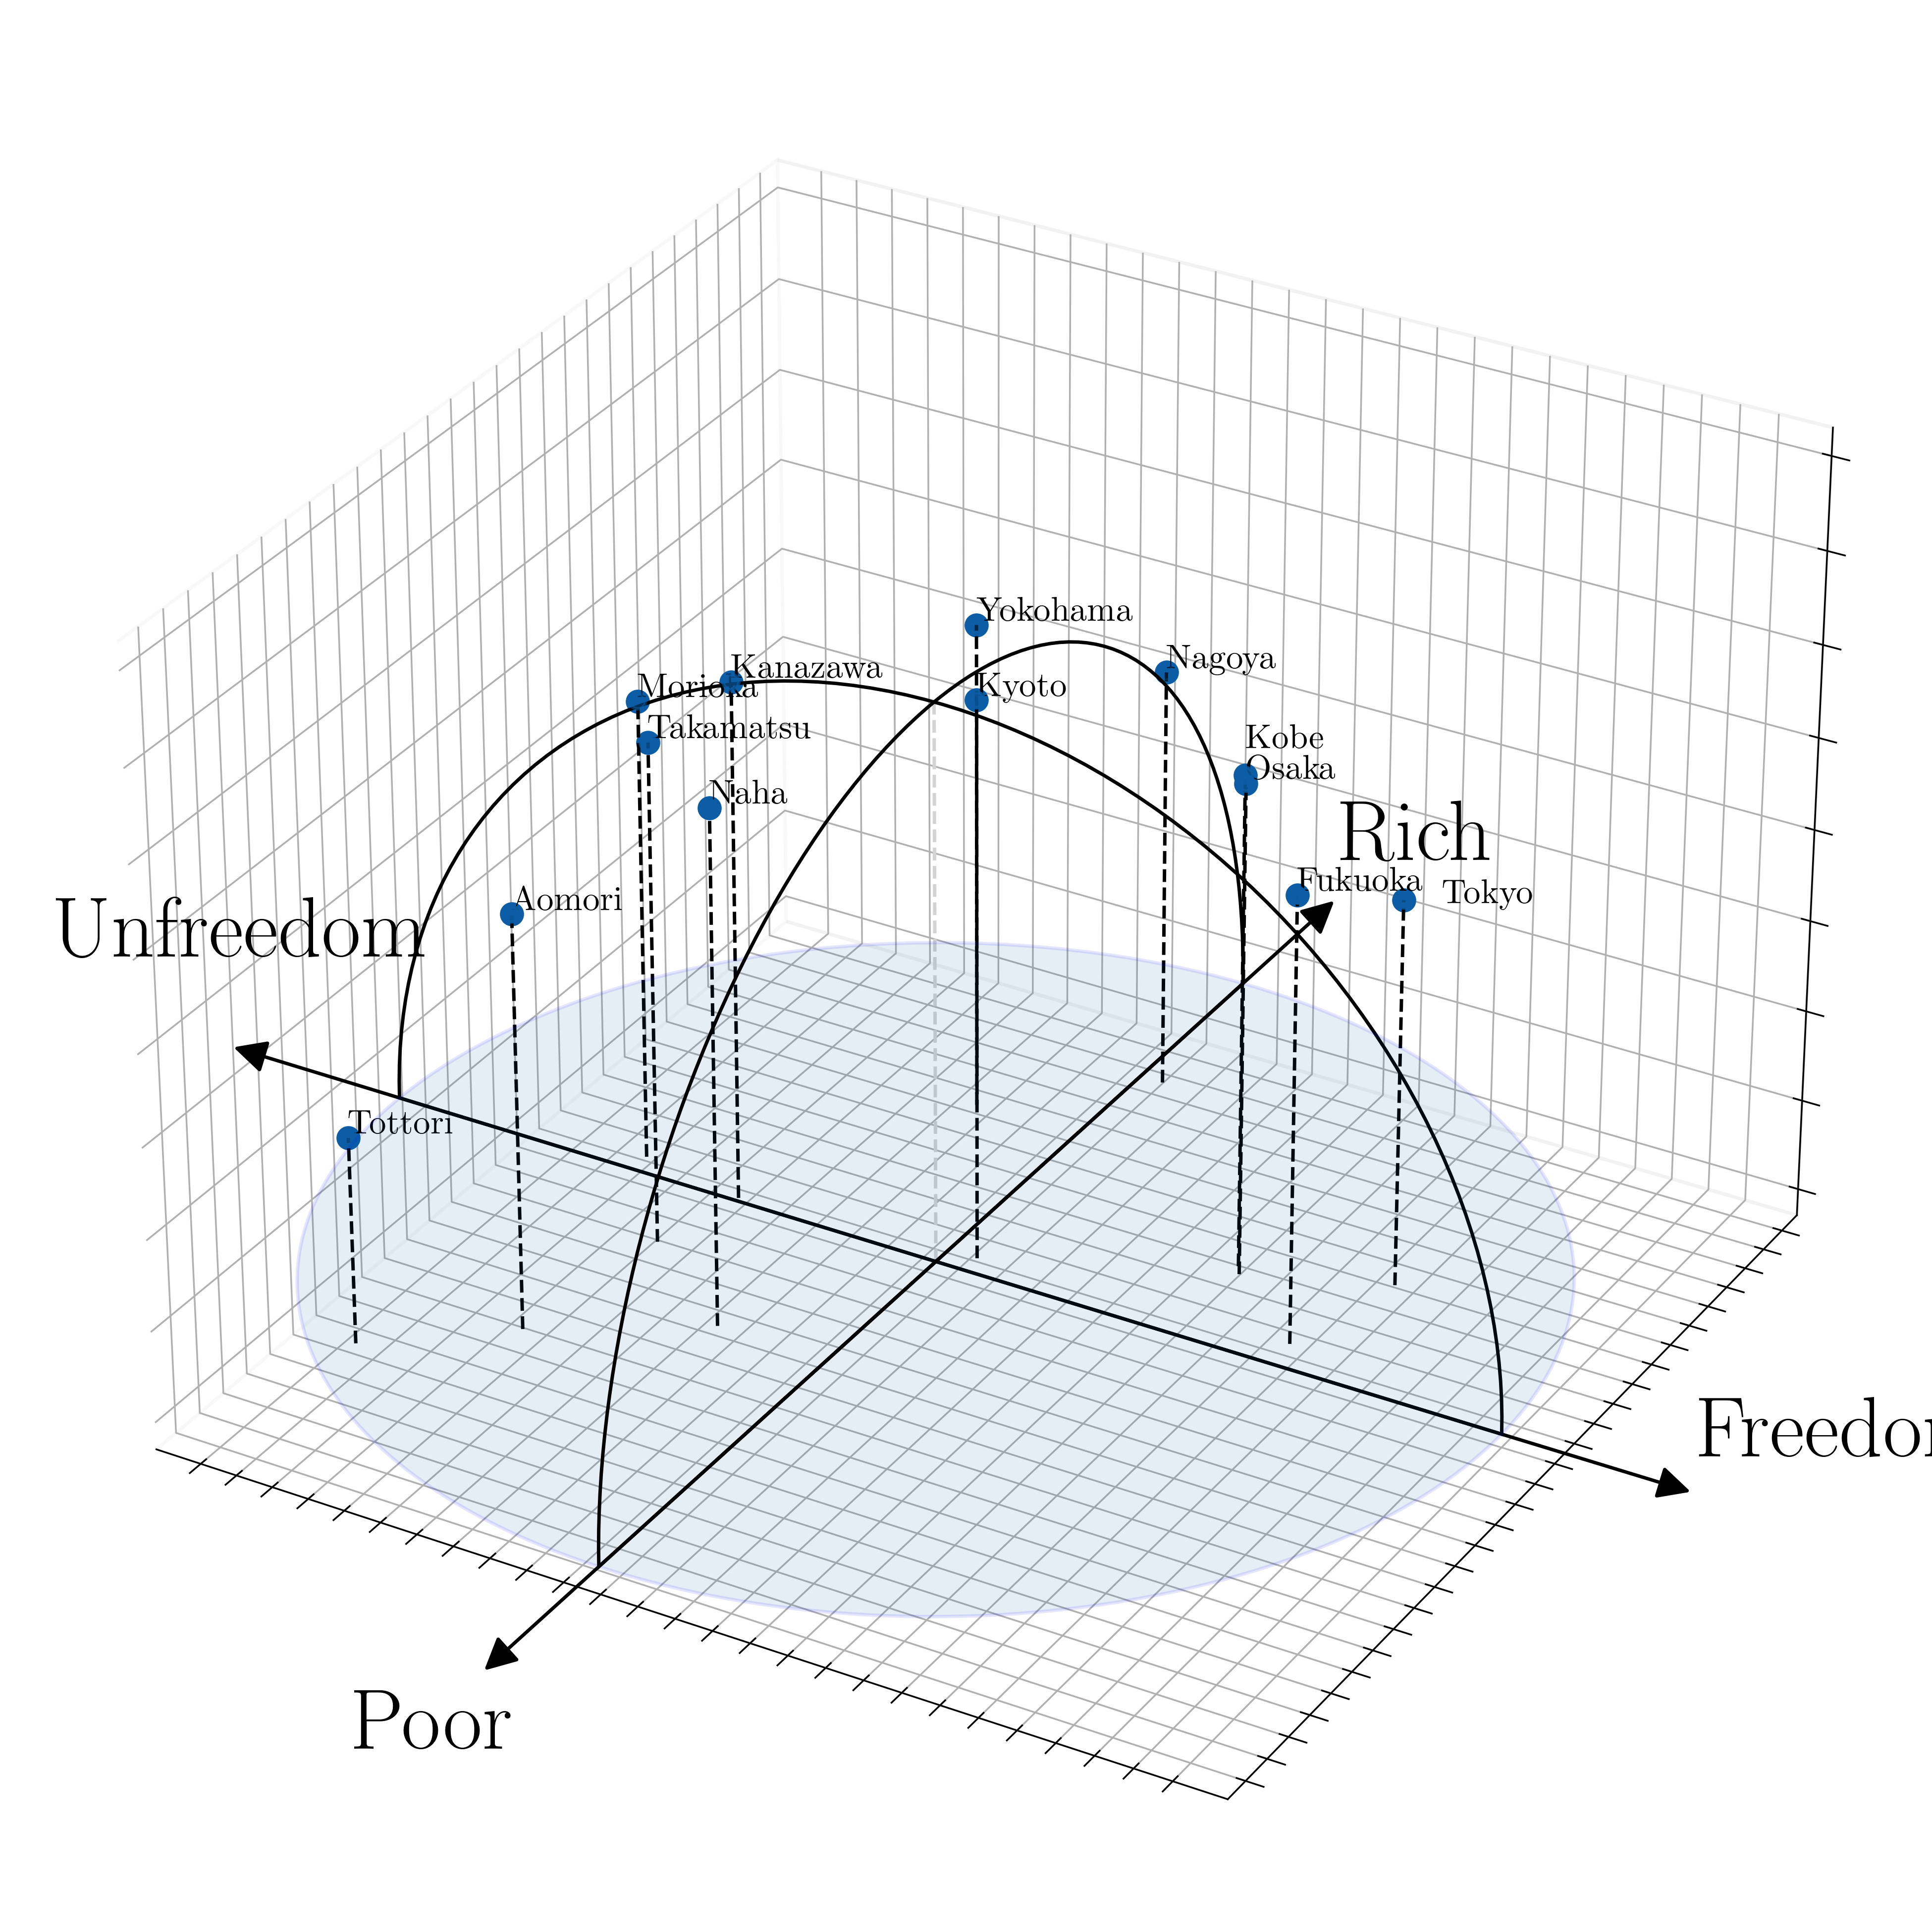
\includegraphics[width=0.55\linewidth]{Figure/rich_poor.png}
                    \caption{単語埋め込みによる意味空間の構築}
                    \label{fig:enter-label}
                \end{figure}
            \end{minipage}
        \end{column}
    \end{columns}
\end{frame}



\end{document}
